\section{Diseño de la base de datos}
\label{dev:sec:diseno_base_datos}

Para estructurar el proyecto, se ha optado por empezar definiendo la base de datos. Diseñar la base de datos inicialmente permite tener una visión general de como se va a estructurar el proyecto y como sus distintas partes se van a relacionar entre sí. Al fin y al cabo, la base de datos es el núcleo de la aplicación, ya que de ella dependen todas las funcionalidades.

En concreto, para el proyecto se ha decidido hacer uso del sistema de gestión de bases de datos PostgreSQL. Esta elección es resultado de la experiencia previa que he tenido con este sistema, ya que he trabajado con él en proyectos anteriores y me he familiarizado con su funcionamiento. Además, PostgreSQL es un sistema de código abierto, lo que significa que es gratuito y se puede utilizar sin restricciones, siendo una solución muy robusta y escalable, lo que lo hace ideal para aplicaciones de gran tamaño, como podría ser esta en un futuro. Por último, es el sistema que mejor se integra con Django, por lo que es la opción más lógica a escoger.

\subsection{Bloques de funcionalidades}
\label{dev:subsec:bloques_funcionalidades}

Antes de empezar a diseñar la base de datos, se deben definir los bloques clave de la aplicación para así poder estructurar los datos de manera que se puedan implementar de la mejor manera posible. Estos bloques van a tener gran relevancia a lo largo del desarrollo, ya que van a definir como se estructura todo: tanto el \textit{backend} como el \textit{frontend}. Consecuentemente, los bloques de funcionalidades que se han definido son los siguientes:

\begin{itemize}
    \item \textbf{Bloque de canales:} La herramienta debe permitir la gestión de los distintos canales de venta en línea. Aunque el usuario no crea ni edita de manera directa los canales de venta, interactúa con ellos, de manera que su información debe estar almacenada en la base de datos.
    \item \textbf{Bloque de pedidos:} La herramienta debe centralizar todos los pedidos de los distintos canales de venta en línea y permitir la gestión de los mismos. Esto incluye la posibilidad de crear, editar y eliminar pedidos, así como de cambiar el estado de los mismos.
    \item \textbf{Bloque de productos:} La herramienta debe permitir la gestión de los productos disponibles en los distintos canales de venta en línea. Esto incluye la posibilidad de crear, editar y eliminar productos de los distintos canales, así como de editar sus atributos, tales como el precio, la descripción y la imagen, entre muchos otros. Además, debe permitir personalizar los atributos de cada producto según el canal de venta, ya que cada canal puede tener sus propios atributos y propiedades.
          % \item \textbf{Bloque de usuarios y autenticación:} La herramienta debe permitir la gestión de los usuarios que pueden acceder a la aplicación. Esto incluye la posibilidad de crear, editar y eliminar usuarios, así como la de asignarles distintos permisos y roles dentro de la aplicación.
\end{itemize}

Con los bloques clave definidos, se puede concluir que la base de datos debe contener cuatro tablas principales: una para los pedidos, otra para los productos y una última para los canales. A partir de aquí, se pueden definir las distintas tablas que van a complementar las principales.

Adicionalmente, dado que para este proyecto la aplicación se presenta como una fase inicial de una desarrollo mucho más grande, que en un futuro podría convertirse en una solución comercializable, es indispensable tener en cuenta la escalabilidad de toda la aplicación. Por este motivo, los tres bloques que a continuación se detallarán han sido diseñados de manera que se puedan ampliar en un futuro sin necesidad de realizar cambios significativos en la base de datos.

\subsubsection{Bloque de canales de venta}

El bloque de canales de venta es el conjunto de tablas y relaciones que almacenan toda la información correspondiente a los distintos canales de venta en línea. El usuario no interactúa directamente con los canales de venta, es decir, no los crea ni los edita, pero sí que interactúa con ellos al sincronizarlos con sus pedidos y productos.

Este bloque es el más claro ejemplo de la escalabilidad de la aplicación y de la base de datos, ya que trata a cada canal de venta como una entidad independiente, lo que permite añadir nuevos canales sin necesidad de realizar cambios a la estructura de la base de datos.

Este bloque está formado únicamente por una tabla, que es la siguiente:
\begin{itemize}
    \item \textbf{Canal de venta [\texttt{marketplace}]:} Esta tabla almacena la información de los distintos canales de venta en línea. Los campos que contiene son los siguientes:
          \begin{itemize}
              \item \texttt{id}: Identificador único del canal de venta. \textit{Clave primaria (entero)}.
              \item \texttt{name}: Nombre del canal de venta. \textit{Cadena de caracteres}.
              \item \texttt{logo\_url}: URL del logo del canal de venta. \textit{Cadena de caracteres}.
              \item \texttt{color}: Color del canal de venta. \textit{Cadena de caracteres}.
              \item \texttt{country}: País del canal de venta. \textit{Entero}.
          \end{itemize}
\end{itemize}

Con la tabla definida, se puede describir el funcionamiento del bloque. El desarrollador de la aplicación puede añadir nuevos canales de venta añadiendo nuevas filas a la tabla. Este enfoque permite que nuevos canales de venta puedan ser añadidos sin necesidad de hacer grandes cambios en la aplicación, pues cada canal de venta es tratado como una entidad independiente. Al añadir un nuevo canal de venta el usuario verá el nuevo canal en la aplicación tal como si fuera uno ya existente, pudiendo sincronizar sus pedidos y productos con él.

\subsubsection{Bloque de pedidos}

El bloque de pedidos es el conjunto de tablas y relaciones que almacenan toda la información correspondiente a los pedidos. En cada pedido es importante almacenar la información de éste, como el estado, la fecha, el método de pago, el canal de venta, entre otros. Además, para saber donde se debe enviar el pedido, es importante almacenar la información del cliente, como su nombre, dirección y teléfono. Por último, también es importante almacenar la información de los productos que componen el pedido, como su nombre, precio y cantidad solicitada.

Conociendo la información que se debe almacenar, se pueden definir las siguientes tablas:

\begin{itemize}
    \item \textbf{Pedido [\texttt{order}]:} Esta tabla almacena la información general de cada pedido. Los campos que contiene son los siguientes:
          \begin{itemize}
              \item \texttt{id}: Identificador único del pedido. \textit{Clave primaria (entero)}.
              \item \texttt{order\_id}: Identificador del pedido en el canal de venta. \textit{Cadena de caracteres}.
              \item \texttt{status}: Estado del pedido (pendiente, enviado, entregado, cancelado). \textit{Entero}.
              \item \texttt{order\_date}: Fecha en la que se realizó el pedido. \textit{Fecha y hora}.
              \item \texttt{total\_price}: Precio total del pedido. \textit{Decimal}.
              \item \texttt{ticket}: Número de ticket del pedido. \textit{Cadena de caracteres}.
              \item \texttt{ticket\_refund}: Número de ticket de la devolución del pedido. \textit{Cadena de caracteres}.
              \item \texttt{pay\_method}: Método de pago del pedido (tarjeta, transferencia, efectivo). \textit{Entero}.
              \item \texttt{package\_quantity}: Cantidad de bultos (paquetes) del pedido. \textit{Entero}.
              \item \texttt{weight}: Peso del pedido. \textit{Decimal}.
              \item \texttt{notes}: Notas del pedido. \textit{Cadena de caracteres}.
              \item \texttt{origin}: Origen del pedido (creado automáticamente, importado, manual). \textit{Entero}.
              \item \texttt{updated\_at}: Fecha de la última actualización del pedido. \textit{Fecha y hora}.
              \item \texttt{carrier\_id}: Identificador del transportista del pedido. \textit{Entero y relación N:1 con la tabla} \texttt{carrier}.
              \item \texttt{customer\_id}: Identificador del cliente del pedido. \textit{Entero y relación N:1 con la tabla} \texttt{customer}.
              \item \texttt{marketplace\_id}: Identificador del canal de venta del pedido. \textit{Entero y relación N:1 con la tabla} \texttt{marketplace}.
          \end{itemize}
    \item \textbf{Cliente [\texttt{customer}]:} Esta tabla almacena la información del cliente. Se divide entre información de facturación e información de envío, ya que es habitual que los canales de venta permitan añadir ambos tipos de información. Los campos que contiene son los siguientes:
          \begin{itemize}
              \item \texttt{id}: Identificador único del cliente. \textit{Clave primaria (entero)}.
              \item \texttt{bill\_phone}: Teléfono de facturación. \textit{Cadena de caracteres}.
              \item \texttt{bill\_email}: Correo electrónico de facturación. \textit{Cadena de caracteres}.
              \item \texttt{bill\_firstname}: Nombre del cliente para la facturación. \textit{Cadena de caracteres}.
              \item \texttt{bill\_lastname}: Apellido del cliente para la facturación. \textit{Cadena de caracteres}.
              \item \texttt{bill\_company}: Empresa del cliente para la facturación. \textit{Cadena de caracteres}.
              \item \texttt{bill\_address}: Dirección de facturación. \textit{Cadena de caracteres}.
              \item \texttt{bill\_city}: Ciudad de facturación. \textit{Cadena de caracteres}.
              \item \texttt{bill\_zipcode}: Código postal de facturación. \textit{Cadena de caracteres}.
              \item \texttt{bill\_country}: País de facturación. \textit{Entero}.
              \item \texttt{ship\_phone}: Teléfono de envío. \textit{Cadena de caracteres}.
              \item \texttt{ship\_email}: Correo electrónico de envío. \textit{Cadena de caracteres}.
              \item \texttt{ship\_firstname}: Nombre del cliente para el envío. \textit{Cadena de caracteres}.
              \item \texttt{ship\_lastname}: Apellido del cliente para el envío. \textit{Cadena de caracteres}.
              \item \texttt{ship\_company}: Empresa del cliente para el envío. \textit{Cadena de caracteres}.
              \item \texttt{ship\_address}: Dirección de envío. \textit{Cadena de caracteres}.
              \item \texttt{ship\_city}: Ciudad de envío. \textit{Cadena de caracteres}.
              \item \texttt{ship\_zipcode}: Código postal de envío. \textit{Cadena de caracteres}.
              \item \texttt{ship\_country}: País de envío. \textit{Entero pequeño}.
          \end{itemize}
    \item \textbf{Artículo [\texttt{orderitem}]:} Esta tabla almacena la información de los productos que componen el pedido. Los campos que contiene son los siguientes:
          \begin{itemize}
              \item \texttt{id}: Identificador único del artículo. \textit{Clave primaria (entero)}.
              \item \texttt{order\_id}: Identificador del pedido al que pertenece el artículo. \textit{Entero y relación N:1 con la tabla} \texttt{order}.
              \item \texttt{marketplace\_product\_id}: Identificador del producto del artículo. \textit{Entero y relación N:1 con la tabla} \texttt{marketplace\_product}.
              \item \texttt{purchase\_price}: Precio del producto en el momento que se adquirió. \textit{Decimal}.
              \item \texttt{quantity}: Cantidad solicitada del producto del artículo. \textit{Entero}.
          \end{itemize}
    \item \textbf{Transportista [\texttt{carrier}]:} Esta tabla almacena la información de los transportistas. Los campos que contiene son los siguientes:
          \begin{itemize}
              \item \texttt{id}: Identificador único del transportista. \textit{Clave primaria (entero)}.
              \item \texttt{name}: Nombre del transportista. \textit{Cadena de caracteres}.
          \end{itemize}
\end{itemize}

Con esto, se puede observar que el bloque está formado por una tabla principal, la de pedidos \texttt{order}, que almacena la información general de cada pedido, y tres tablas complementarias: la de clientes \texttt{customer}, que almacena la información del cliente, la de artículos \texttt{orderitem}, que almacena la información de los productos que componen el pedido, y la de transportistas \texttt{carrier}, que almacena la información de los transportistas.

Si bien es cierto que la tabla de cliente podría parecer ser redundante, pues toda la información del cliente \texttt{customer} podría almacenarse directamente en la tabla de pedidos, se ha optado por crear una tabla independiente para poder reutilizar la información del cliente en otros pedidos. De esta manera, si un cliente realiza varios pedidos, su información solo se almacena una vez, lo que permite reducir el espacio de almacenamiento y mejorar la eficiencia de la base de datos, además de permitir hacer filtros, búsquedas y análisis de datos más eficientes; opciones que podrían ser muy útiles en un futuro si se quiere implementar una funcionalidad de análisis de datos.

Por otro lado, la tabla de artículos \texttt{orderitem} no almacena la información del producto, sino que relaciona el pedido con el producto del canal de venta. Esta práctica permite, al igual que con la tabla de clientes, reutilizar la información del producto en otros pedidos, lo que reduce el espacio de almacenamiento y mejora la eficiencia de la base de datos. Además, este enfoque permite que en un futuro se puedan hacer herramientas de análisis de datos, ya que se puede relacionar el pedido con el producto del canal de venta y obtener información sobre las ventas de cada producto. El único campo que almacena información del producto es el precio de compra, ya que es importante conocer el precio al que se adquirió el producto en el momento de la compra al ser un dato esencial muy cambiante.

Por último, la tabla de transportista \texttt{carrier} tiene un funcionamiento similar al de la tabla de canales de venta, ya que cada transportista es tratado como una entidad independiente. Esto permite al desarrollador añadir nuevos transportistas sin necesidad de hacer grandes cambios en la aplicación, y al usuario ver los nuevos transportistas en la aplicación tal como si fueran uno ya existente, pudiendo asignarlos a los pedidos.

De esta manera, al generarse un nuevo pedido se añadiría una nueva fila a la tabla de pedidos \texttt{order}, una nueva fila a la tabla de clientes \texttt{customer} (si el cliente no existe ya) y tantas filas a la tabla de artículos \texttt{orderitem} como tipos de productos que el cliente haya adquirido.

\subsubsection{Bloque de productos}

El bloque de productos es el conjunto de tablas y relaciones que conforman y almacenan toda la información correspondiente a los productos. Es sin duda el bloque más complejo de la aplicación, ya que cada canal de venta puede tener sus propios productos y cada producto puede tener sus propios atributos o propiedades.

Así pues, primero de todo se debe entender como se puede relacionar un producto con un canal de venta y como se pueden gestionar los distintos atributos de cada uno de ellos para que la aplicación pueda ser lo más escalable y flexible posible. Para ello, se ha optado por crear las tablas siguientes:

\begin{itemize}
    \item \textbf{Producto [\texttt{product}]:} Esta tabla almacena la información general de cada producto. Los campos que contiene son los siguientes:
          \begin{itemize}
              \item \texttt{id}: Identificador único del producto. \textit{Clave primaria (entero)}.
              \item \texttt{name}: Nombre del producto. \textit{Cadena de caracteres}.
              \item \texttt{sku}: Código SKU del producto. \textit{Cadena de caracteres}.
              \item \texttt{reference}: Referencia del producto. \textit{Cadena de caracteres}.
              \item \texttt{price}: Precio del producto. \textit{Decimal}.
              \item \texttt{stock}: Cantidad de stock del producto. \textit{Entero}.
              \item \texttt{parent\_id}: Identificador del producto padre, en caso de que el producto sea una variante de otro producto. Si el producto es padre o no tiene hijos, el campo está vacío. \textit{Entero y relación N:1 con la misma tabla} \texttt{product}.
              \item \texttt{image}: URL de la imagen del producto. \textit{Cadena de caracteres}.
          \end{itemize}
\end{itemize}

Como se puede observar, el bloque de productos se puede dividir en dos capas: una primera capa (capa  \texttt{product}) que almacena la información del producto, sin entrar a una vinculación con ningún canal de venta, y una segunda capa (capa  \texttt{marketplaceproduct}) que relaciona el producto con el canal de venta. Ambas capas son bastante similares, ya que tienen una tabla principal que almacena el producto en sí, una tabla complementaria que almacena los tipos de atributos que se pueden asignar a los productos y otra tabla adicional que almacena los valores de los atributos de cada producto. \textcolor{red}{De esta manera, a partir de ahora, los productos vinculados a un canal de venta van a ser llamados \textit{marketplace products} y los productos sin vinculación a ningún canal de venta van a ser llamados \textit{products}.}

Un producto \texttt{product} puede tener distintos tipos de atributos, como el color, la talla, el peso, etc. Por este motivo, se ha optado por crear una tabla de tipos de atributos \texttt{productattributetype} que almacena los distintos tipos de atributos que se pueden asignar a los productos. Con esto, el desarrollador puede añadir nuevos tipos de atributos sin necesidad de hacer cambios en la lógica de la aplicación. No obstante, una vez se ha definido el tipo de atributo, se debe asignar un valor a este tipo de atributo para cada producto. Por este motivo, se ha creado una tabla de valores de atributos \texttt{productattribute} que almacena los valores de los atributos de cada producto. Así pues, para cada capa habrá un total de tres tablas: una para los productos, otra para los tipos de atributos y una última para los valores de los atributos.

Para vincular el producto con el canal de venta, se ha creado una tabla de los productos del canal de venta \texttt{marketplaceproduct}. Esta tabla tiene una relación N:1 con la tabla de productos \texttt{product}, lo que significa que un producto puede estar vinculado a varios productos de canales de venta, pero un producto de canal de venta solo puede tener un único producto. De esta manera, se permite que un producto pueda ser vendido en varios canales de venta sin necesidad de duplicar la información del producto. Adicionalmente y de manera análoga a la primera capa, como cada canal de venta puede tener sus propios atributos, se ha creado una tabla de tipos de atributos del canal de venta \texttt{marketplaceproductattributetype} que almacena los distintos tipos de atributos que se pueden asignar a los productos del canal de venta. Consecuentemente, también se ha creado una tabla de valores de atributos del canal de venta \texttt{marketplaceproductattribute} que almacena los valores de los atributos de cada producto del canal de venta.

De esta manera, tanto los atributos de los productos como los atributos de los productos del canal de venta forman con sus respectivas tablas de productos una relación N:M, lo que significa que un producto puede tener varios atributos y un atributo puede pertenecer a varios productos, sin la posibilidad de dos tipos de atributos iguales puedan existir en un mismo producto.

Adicionalmente, cabe remarcar el motivo por el que se separan los atributos de los productos y los atributos de los productos del canal de venta. Cada canal de venta define sus propios atributos para los productos, por lo que es necesario diferenciarlos. Por ejemplo, un canal de venta puede tener un atributo de color y otro de talla, mientras que otro canal de venta puede tener un atributo de peso y otro de dimensiones. Además, cada canal de venta puede tener sus propios valores para los mismos atributos, como por ejemplo el color rojo o el color azul. Por este motivo, se ha optado por crear dos capas diferenciadas para los productos y los productos del canal de venta.

Con esta estructura discutida, en el esquema \ref{fig:products_db_diagram} se puede observar un caso de uso para lograr un mayor en entendimiento de como funcionaría el flujo de creación de un producto y su vinculación con un canal de venta. En concreto, el esquema muestra como se crea un producto y se vincula a un canal de venta, añadiendo los distintos tipos de atributos.

\begin{figure}[H]
    \centering
    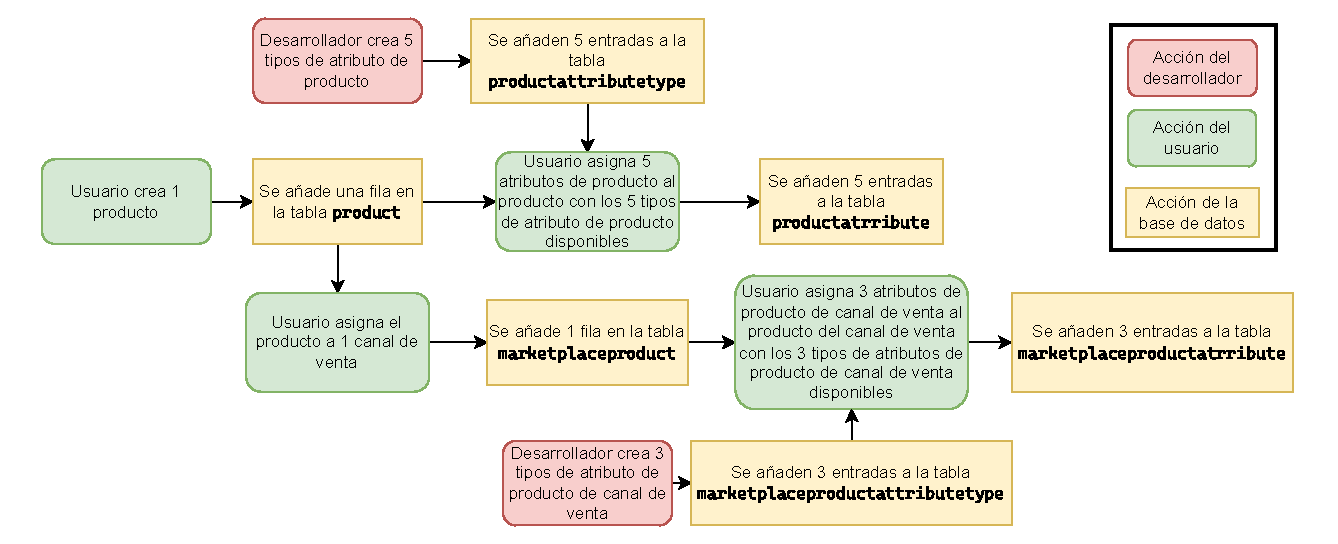
\includegraphics[width=0.8\textwidth]{figures/design_develop/products_db_diagram.pdf}
    \caption{Esquema de flujo de creación de un producto y su vinculación con un canal de venta.}
    \label{fig:products_db_diagram}
\end{figure}

Por último, en las tablas de atributos, tanto de productos como de productos del canal de venta, se ha decidido hacer una columna para cada tipo de valor, es decir, una columna por si el valor es un número, una cadena de caracteres, una fecha, etc. Dichas columnas van acompañadas otra columna, llamada \texttt{data\_type} que indica el tipo de valor, de manera que se puede saber que columna contiene el valor del atributo. El tipo de atributo también tiene una columna \texttt{data\_type}, de manera que deben ser ambos coincidentes. Así pues, a modo de ejemplo, si el tipo de atributo es "Talla", el \texttt{data\_type} será "Integer" y su entrada tendrá todas las columnas vacías exceptuando la columna \texttt{data\_int}.

\textcolor{red}{\textbf{Falta hacer una revisión más exhaustiva}}

% \subsubsection{Bloque de usuarios y autenticación}
% \label{subsubsec:usuarios_autenticacion}

% El bloque de usuarios y autenticación es el conjunto de tablas y relaciones que almacenan toda la información correspondiente a los usuarios que pueden acceder a la aplicación. Este bloque es esencial para la gestión de la aplicación, ya que permite controlar quién puede acceder a la aplicación y qué permisos tiene cada usuario. Un usuario no debe poder ver ni interactuar con los pedidos y productos de otros usuarios, por lo que es necesario implementar un sistema de autenticación y autorización que permita controlar el acceso a la aplicación y mostrar únicamente la información que le corresponde a cada uno.

% Hacer un buen sistema de usuarios o autenticación es normalmente una tarea muy compleja, ya que se deben tener en cuenta muchos aspectos, como la seguridad, la privacidad y los permisos, entre muchas otras cosas. Por este motivo, es una práctica bastante común y recomendable utilizar un sistema de gestión de usuarios ya existente e integrarlo y adaptarlo a las necesidades de la aplicación. Al considerarse una buena práctica, al menos para aplicaciones de tamaño pequeño o mediano, existen múltiples sistemas, como pueden ser Auth0, Firebase Authentication o Amazon Cognito. Sin embargo, como en este proyecto se ha optado por utilizar Django, se ha decidido utilizar su propio sistema de gestión de usuarios que este ofrece nativamente, ya que es un sistema robusto, seguro y fácil de integrar. Si bien es cierto que no es un sistema tan flexible como los mencionados anteriormente, es más que suficiente para las necesidades de la aplicación, al menos en un principio, y permite una integración rápida y sencilla con el \textit{backend}.

% Las funcionalidades que ofrece el sistema de autenticación de Django son las siguientes:

% \begin{itemize}
%     \item Registro de usuarios: Permite a los usuarios registrarse en la aplicación, creando una cuenta con un nombre de usuario y una contraseña.
%     \item Inicio de sesión y cierre de sesión: Permite a los usuarios iniciar sesión en la aplicación con su nombre de usuario y contraseña, y cerrar sesión cuando lo deseen.
%     \item Cambios y recuperación de contraseñas: Permite a los usuarios cambiar su contraseña y recuperar su cuenta en caso de que la hayan olvidado.
%     \item Gestión de permisos y grupos de usuarios: Permite asignar permisos y roles a los usuarios, de manera que se pueda controlar qué funcionalidades pueden utilizar y qué datos pueden ver. Esto es especialmente útil para aplicaciones que tienen distintos tipos de usuarios, como administradores, clientes o empleados.
%     \item Control de acceso: Permite controlar el acceso a las distintas funcionalidades de la aplicación, de manera que solo los usuarios autorizados puedan acceder a ellas.
% \end{itemize}

% Con las funcionalidades definidas, se pueden estudiar las tablas que Django va a utilizar para almacenar toda la información que permita realizar estas funcionalidades. En concreto, el sistema de autenticación hace uso las siguientes tablas:

% \begin{itemize}
%     \item \textbf{Usuario [\texttt{auth\_user}]:} Esta tabla almacena la información de los usuarios. Los campos que contiene son los siguientes:
%           \begin{itemize}
%               \item \texttt{id}: Identificador único del usuario. \textit{Clave primaria (entero)}.
%               \item \texttt{username}: Nombre de usuario del usuario. \textit{Cadena de caracteres}.
%               \item \texttt{password}: Contraseña del usuario. \textit{Cadena de caracteres}.
%               \item \texttt{email}: Correo electrónico del usuario. \textit{Cadena de caracteres}.
%               \item \texttt{first\_name}: Nombre del usuario. \textit{Cadena de caracteres}.
%               \item \texttt{last\_name}: Apellido del usuario. \textit{Cadena de caracteres}.
%               \item \texttt{is\_active}: Indica si el usuario está activo o no. \textit{Booleano}.
%               \item \texttt{is\_staff}: Indica si el usuario es un miembro del personal o no. Esto permite que el usuario pueda acceder al panel de administración de Django. \textit{Booleano}.
%               \item \texttt{is\_superuser}: Indica si el usuario es un superusuario o no. Esto permite que el usuario tenga todos los permisos y pueda acceder a todas las funcionalidades de la aplicación. \textit{Booleano}.
%               \item \texttt{last\_login}: Fecha y hora del último inicio de sesión del usuario. Este campo es útil para saber cuándo fue la última vez que el usuario accedió a la aplicación. Si el usuario nunca ha iniciado sesión, este campo estará vacío. \textit{Fecha y hora}.
%               \item \texttt{date\_joined}: Fecha y hora en la que el usuario se registró en la aplicación. Este campo es útil para saber cuándo se creó la cuenta del usuario. \textit{Fecha y hora}.
%           \end{itemize}
%     \item \textbf{Grupo [\texttt{auth\_group}]:} Esta tabla almacena los grupos de usuarios. Los campos que contiene son los siguientes:
%           \begin{itemize}
%               \item \texttt{id}: Identificador único del grupo. \textit{Clave primaria (entero)}.
%               \item \texttt{name}: Nombre del grupo. \textit{Cadena de caracteres}.
%           \end{itemize}
%     \item \textbf{Permiso [\texttt{auth\_permission}]:} Esta tabla almacena los permisos que pueden ser asignados a los usuarios y grupos. Los campos que contiene son los siguientes:
%           \begin{itemize}
%               \item \texttt{id}: Identificador único del permiso. \textit{Clave primaria (entero)}.
%               \item \texttt{name}: Nombre del permiso. \textit{Cadena de caracteres}.
%               \item \texttt{codename}: Código del permiso. Este campo es único y se utiliza para identificar el permiso en la aplicación. \textit{Cadena de caracteres}.
%           \end{itemize}
%     \item \textbf{Permiso de grupo [\texttt{auth\_group\_permissions}]:} Esta tabla almacena la relación entre los grupos y los permisos que tienen asignados. Así pues, esta tabla relaciona las tablas \texttt{auth\_group} y \texttt{auth\_permission}. Los campos que contiene son los siguientes:
%           \begin{itemize}
%               \item \texttt{id}: Identificador único de la relación. \textit{Clave primaria (entero)}.
%               \item \texttt{group\_id}: Identificador del grupo al que pertenece el permiso. Este campo es una relación N:1 con la tabla \texttt{auth\_group}. \textit{Entero}.
%               \item \texttt{permission\_id}: Identificador del permiso asignado al grupo. Este campo es una relación N:1 con la tabla \texttt{auth\_permission}. \textit{Entero}.
%           \end{itemize}
%     \item \textbf{Permiso de usuario [\texttt{auth\_user\_user\_permissions}]:} Esta tabla almacena la relación entre los usuarios y los permisos que tienen asignados. Consecuentemente, la tabla actúa como tabla intermedia entre las tablas \texttt{auth\_user} y \texttt{auth\_permission}. Los campos que contiene son los siguientes:
%           \begin{itemize}
%               \item \texttt{id}: Identificador único de la relación. \textit{Clave primaria (entero)}.
%               \item \texttt{user\_id}: Identificador del usuario al que pertenece el permiso. Este campo es una relación N:1 con la tabla \texttt{auth\_user}. \textit{Entero}.
%               \item \texttt{permission\_id}: Identificador del permiso asignado al usuario. Este campo es una relación N:1 con la tabla \texttt{auth\_permission}. \textit{Entero}.
%           \end{itemize}
%     \item \textbf{Usuario de grupo [\texttt{auth\_user\_groups}]:} Esta tabla almacena la relación entre los usuarios y los grupos a los que pertenecen. De esta manera, actúa como tabla intermedia entre las tablas \texttt{auth\_user} y \texttt{auth\_group}. Los campos que contiene son los siguientes:
%           \begin{itemize}
%               \item \texttt{id}: Identificador único de la relación. \textit{Clave primaria (entero)}.
%               \item \texttt{user\_id}: Identificador del usuario al que pertenece el grupo. Este campo es una relación N:1 con la tabla \texttt{auth\_user}. \textit{Entero}.
%               \item \texttt{group\_id}: Identificador del grupo al que pertenece el usuario. Este campo es una relación N:1 con la tabla \texttt{auth\_group}. \textit{Entero}.
%           \end{itemize}
%     \item \textbf{Sesión [\texttt{django\_session}]:} Esta tabla almacena las sesiones de los usuarios. Los campos que contiene son los siguientes:
%           \begin{itemize}
%               \item \texttt{session\_key}: Clave única de la sesión. Este campo es único y se utiliza para identificar la sesión en la aplicación. \textit{Cadena de caracteres}.
%               \item \texttt{session\_data}: Datos de la sesión. Este campo almacena los datos de la sesión en formato JSON. \textit{Cadena de caracteres}.
%               \item \texttt{expire\_date}: Fecha de expiración de la sesión. Este campo indica cuándo caduca la sesión y se elimina automáticamente. \textit{Fecha y hora}.
%           \end{itemize}
% \end{itemize}

% Con las siete tablas definidas, es necesario explicar el funcionamiento de cada una de ellas y como se relacionan entre sí. En primer lugar, todo parte de la tabla de usuarios \texttt{auth\_user}, que almacena la información de estos, y de la tabla de permisos \texttt{auth\_permission}, que almacena los permisos que pueden ser asignados. A partir de aquí, existen dos maneras de asignar permisos a los usuarios:

% \begin{itemize}
%     \item \textbf{Asignación directa:} Se pueden asignar permisos directamente a los usuarios, lo que significa que el usuario tendrá acceso a las funcionalidades y datos correspondientes a esos permisos. Este enfoque es útil para asignar permisos a usuarios individuales, lo que puede resultar necesario en algunos casos.
%     \item \textbf{Asignación a través de grupos:} Se pueden crear grupos de usuarios y asignarles permisos, lo que significa que todos los usuarios del grupo tendrán acceso a las funcionalidades y datos correspondientes a esos permisos. Este segundo enfoque es útil para asignar permisos a un grupo de usuarios, lo que puede resultar más eficiente y fácil de gestionar.
% \end{itemize}

% Para la asignación directa, se utiliza la tabla \texttt{auth\_user\_user\_permissions}, que relaciona los usuarios con los permisos que tienen asignados. De esta manera, la tabla relaciona las tablas \texttt{auth\_user} y \texttt{auth\_permission}. Cada permiso que se le asigna a un usuario representará una instancia de la tabla. Gracias a esta tabla, se pueden asignar permisos a los usuarios de manera individual, lo que permite un control más granular sobre los permisos de cada usuario.

% Por otro lado, para la asignación a través de grupos, se utilizan las tablas \texttt{auth\_group} y \texttt{auth\_group\_permissions}. La primera almacena los grupos de usuarios y la segunda relaciona los grupos con los permisos que tienen asignados, mediante la relación entre las tablas \texttt{auth\_group} y \texttt{auth\_permission}. Cada permiso que se le asigna a un grupo representará una instancia de la tabla. De esta manera, se pueden crear grupos de usuarios y asignarles permisos, lo que permite un control más eficiente sobre los permisos de los usuarios, pues es mucho más óptimo asignar permisos a un grupo que asignar permisos usuario por usuario.

% No obstante, para asignar los usuarios a los grupos, se utiliza la tabla \texttt{auth\_user\_groups}, que relaciona los usuarios con los grupos a los que pertenecen mediante la relación entre las tablas \texttt{auth\_user} y \texttt{auth\_group}. De esta manera, se pueden asignar usuarios a grupos y, por tanto, asignarles los permisos correspondientes a esos grupos.

% Por último, es importante mencionar como se guarda la contraseña de los usuarios en la base de datos. Idealmente, cualquier persona que pueda llegar a tener acceso a la base de datos, ya sea un desarrollador, un administrador o un atacante, no debería poder acceder a las contraseñas de los usuarios. Por este motivo, las contraseñas no se guardan en texto plano, sino que se almacenan de manera segura utilizando un algoritmo de encriptación. La encriptación de contraseñas es una de aquellas prácticas donde uno no deber reinventar la rueda, ya que existen múltiples algoritmos de encriptación seguros y probados. En este caso, Django utiliza el algoritmo PBKDF2 para realizar la encriptación, guardando la contraseña en el formato siguiente:

% \begin{center}
%     \texttt{<algoritmo>\$<número de iteraciones>\$<salto>\$<hash>}
% \end{center}



\begin{figure} [H]
    \centering
    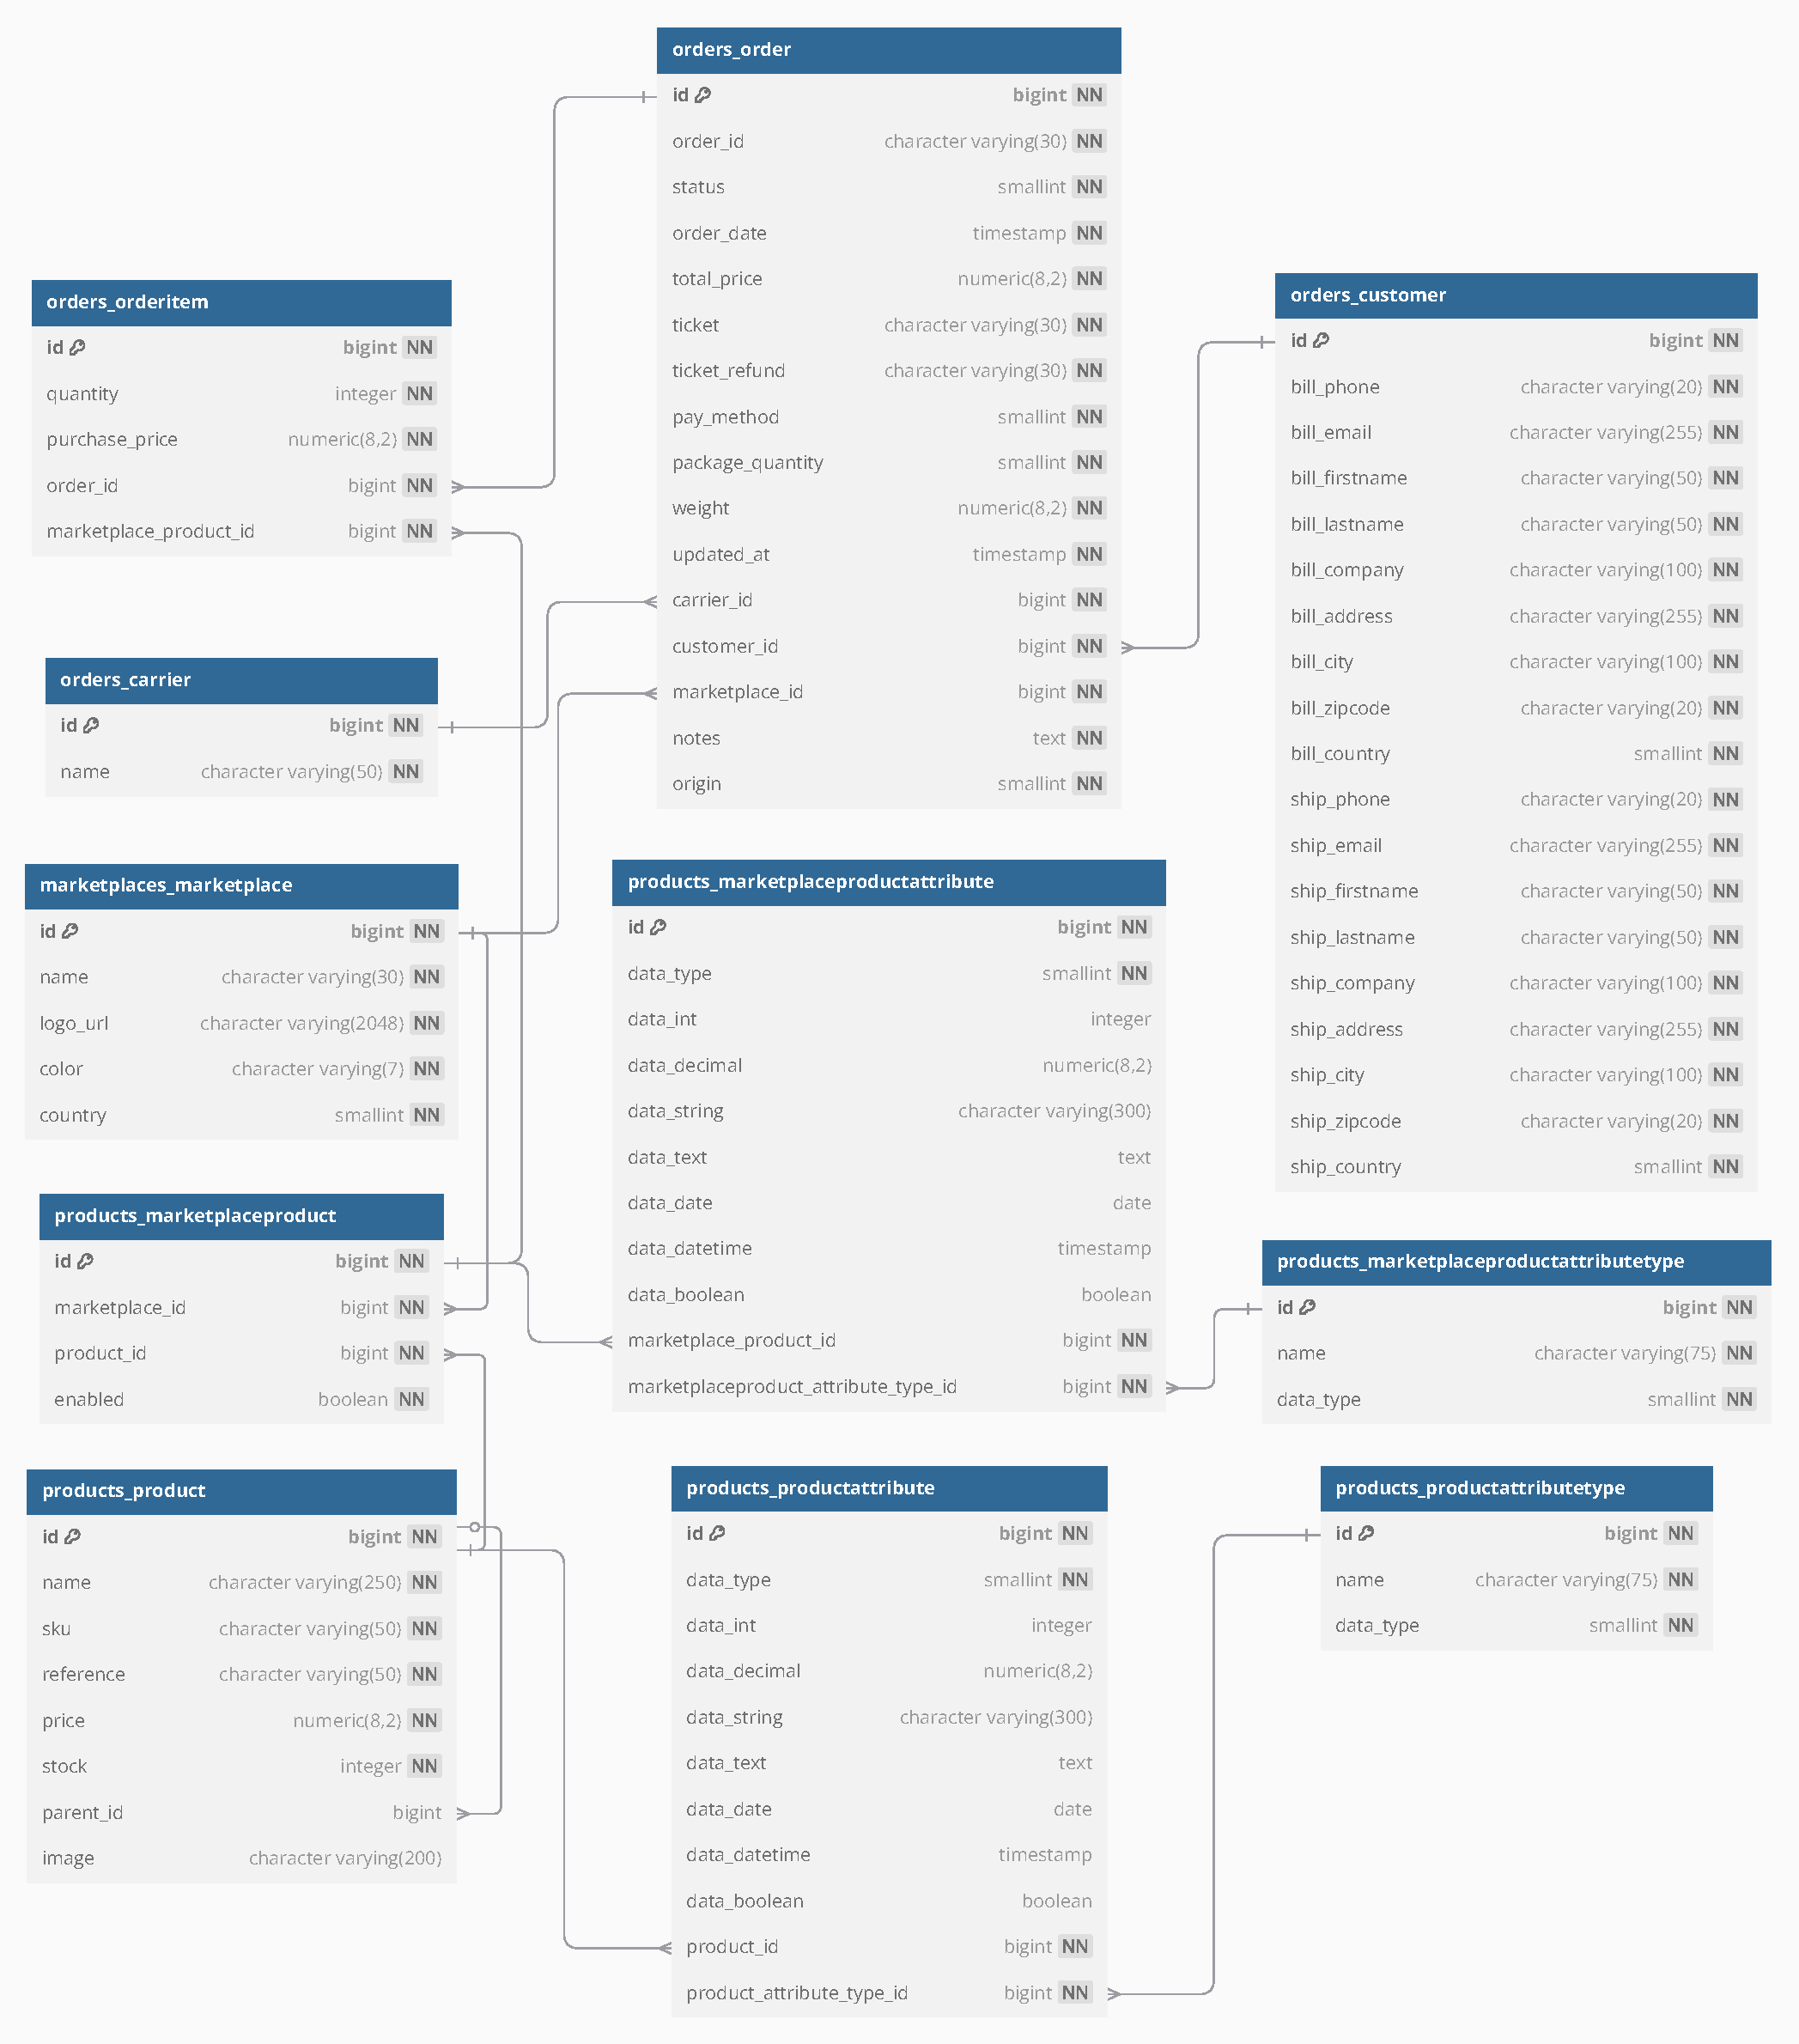
\includegraphics[width=0.98\textwidth]{figures/design_develop/database_diagram.pdf}
    \caption{Diagrama de la base de datos}
    \label{fig:diagrama_base_datos}
\end{figure}